\chapter{The \textit{KsFinder} impact on $M_{bc}$, $\Delta E$ and vertex positions.}


%\textit{KsFinder} largely reduce the combinatorial background of $B^0$ by improving $K_S^0$ purity. 
\begin{comment}
\begin{figure}[htpb]
\centering
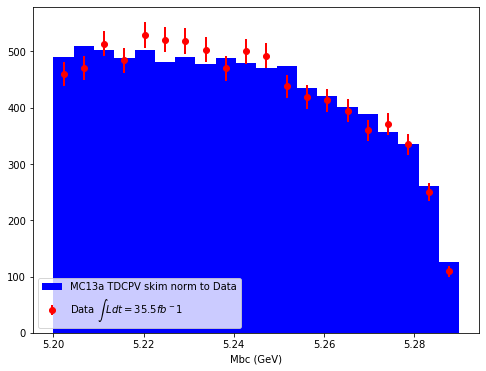
\includegraphics[width=0.7\linewidth]{mbc-noks}
\caption{$M_{bc}$ distribution in data(red) and MC(blue) without $K_S^0$ finder}
\end{figure}
\begin{figure}[htpb]
\centering
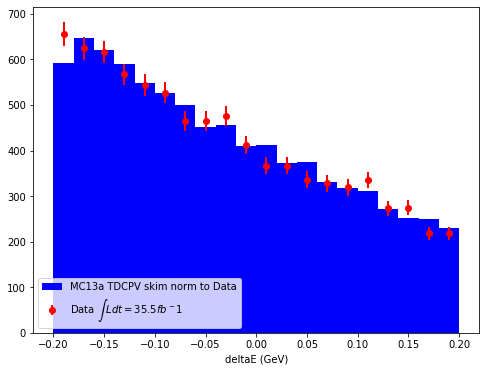
\includegraphics[width=0.7\linewidth]{dE-noks}
\caption{$\Delta{E}$ distribution in data(red) and MC(blue) without $K_S^0$ finder}
\end{figure}
\end{comment}
\textit{KsFinder} provides a classification variable \textit{FBDT\_Ks} to be used as a cut to improve the purity of the $K_S^0$ and $B^0$.
Thus, it's essential to check the potential impact on $M_{bc}$ and $\Delta E$, as well as vertex positions on $z$-axis of $B^0$ after applying \textit{KsFinder}. The $K_S^0$ classification uses information such as invariant mass and decay vertex positions which may propagate bias into $B^0$ signal extraction, eventually may affect the measurement of $\it{CP}$ parameters.

For $K_S^0$ candidates with full SVD hits from their daughter pion tracks, the \textit{KsFinder} can perform a better classification on wether it's a true $K_S^0$ or not, compared to those $K_S^0$ candidates with less SVD hits information. This is because the tracking quality and invariant mass from the fit is highly dependent on the SVD hits information, which plays an important role in calculating input variables used in the \textit{KsFinder}. For example, a true $K_S^0$ is more likely to be wrongly classified if all of its daughter pions have no SVD hits, so the reconstruction can only be done by using 6 CDC-only tracks. Rejecting these candidates might introduce biases. Therefore, given each type of $B^0$ based on how many CDC-only tracks it has in the final states, the comparison on $M_{bc}$ and $\Delta{E}$ with or without \textit{KsFinder} is performed by fitting the distribution in \textit{signal MC}. $M_{bc}$ and $\Delta{E}$ are modeled by signal and double Gaussian functions, respectively. Comparing corresponding fit results, no clear bias on $M_{bc}$ and $\Delta{E}$ is found by using \textit{KsFinder} where fit results are agreed well within one standard deviation. The fit results are shown in Figure \ref{fig:mbc_bias} and \ref{fig:de_bias}. 
 
 \begin{figure}[htpb]
 	\centering
 	\includegraphics[width=0.9\linewidth]{mbc_noKs}
 	\includegraphics[width=0.9\linewidth]{mbc_Ks}
 	\caption{$M_{bc}$ distribution based on the number of CDC-only tracks in final states. Top: no \textit{KsFinder} used; Bottom: \textit{KsFinder} used. The $\mu$ and $\sigma$ are the mean and standard deviation of the Gaussian function.}
 	\label{fig:mbc_bias}
 \end{figure}
 \begin{figure}[htpb]
	\centering
	\includegraphics[width=0.9\linewidth]{dE_noKs}
	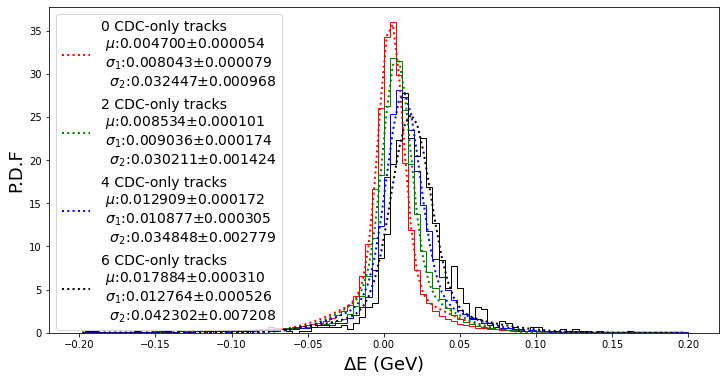
\includegraphics[width=0.9\linewidth]{dE_Ks}
	\caption{$\Delta{E}$ distribution based on the number of CDC-only tracks in final states. Top: no \textit{KsFinder}; Bottom: \textit{KsFinder} used. The $\mu$ is the common mean for double Gaussian. The $\sigma_1$ and $\sigma_2$ are the standard deviations of the Gaussian function.}
	\label{fig:de_bias}
\end{figure}

Similar to the comparison of $M_{bc}$ and $\Delta{E}$, the $z$ direction vertex position and the vertex position difference $\Delta z$ between $\it{CP}$ and tag sides are also checked, in which no clear bias are found either. The $z$ and $\Delta z$ are modeled using single Gaussian with the same mean but different standard deviation. The results are shown in Figure \ref{fig:bias-z} and \ref{fig:bias-zerr}. It is obvious that in Figure \ref{fig:bias-z}, the $\it{CP}$-side resolution of vertex on $z$-axis is wider when the final states of $B^0$ have more CDC-only tracks, especially when all the tracks only contains CDC hits (6 CDC-only tracks).

\begin{figure}[htpb]
	\centering
	\includegraphics[width=0.9\linewidth]{z_noKs}
	\includegraphics[width=0.9\linewidth]{z_Ks}
	\caption{$\Delta z$ distribution based on the number of CDC-only tracks in final states. Top: no \textit{KsFinder}; Bottom: \textit{KsFinder} used. The $\mu$ and $\sigma$ are the mean and standard deviation of the Gaussian function.}
	\label{fig:bias-z}
\end{figure}
\begin{figure}[htpb]
	\centering
	\includegraphics[width=0.9\linewidth]{dz_noKs}
	\includegraphics[width=0.9\linewidth]{dz_Ks}
	\caption{$\Delta z$ distribution based on th number of CDC-only tracks in final states. Top: no \textit{KsFinder}; Bottom: \textit{KsFinder} used. The $\mu$ and $\sigma$ are the mean and standard deviation of each Gaussian function.}
	\label{fig:bias-zerr}
\end{figure}
Above all, no clear appearance of bias on $M_{bc}$ and $\Delta E$ distributions, as well as vertex positions from using \textit{KsFinder} has been found, \textit{KsFinder} may implement a small shift on the vertex position which is negligible compared to the large statistical uncertainty due to the current low luminosity. Hence, there's no correction on these observables are applied in this analysis, and the systematic uncertainty from \textit{KsFinder} is evaluated by taking into account of $R_{B^0}$ in signal fraction calculation which comes from the potential discrepancy of \textit{KsFinder} responses among data and MC. 